\section*{Aufgabe 2 -- Risikobewertung}

Unsere Tabelle zur Risikobewertung ist auch zu finden in \emph{Aufgabe2Tabelle.pdf} zu finden.

\hskip-3.0cm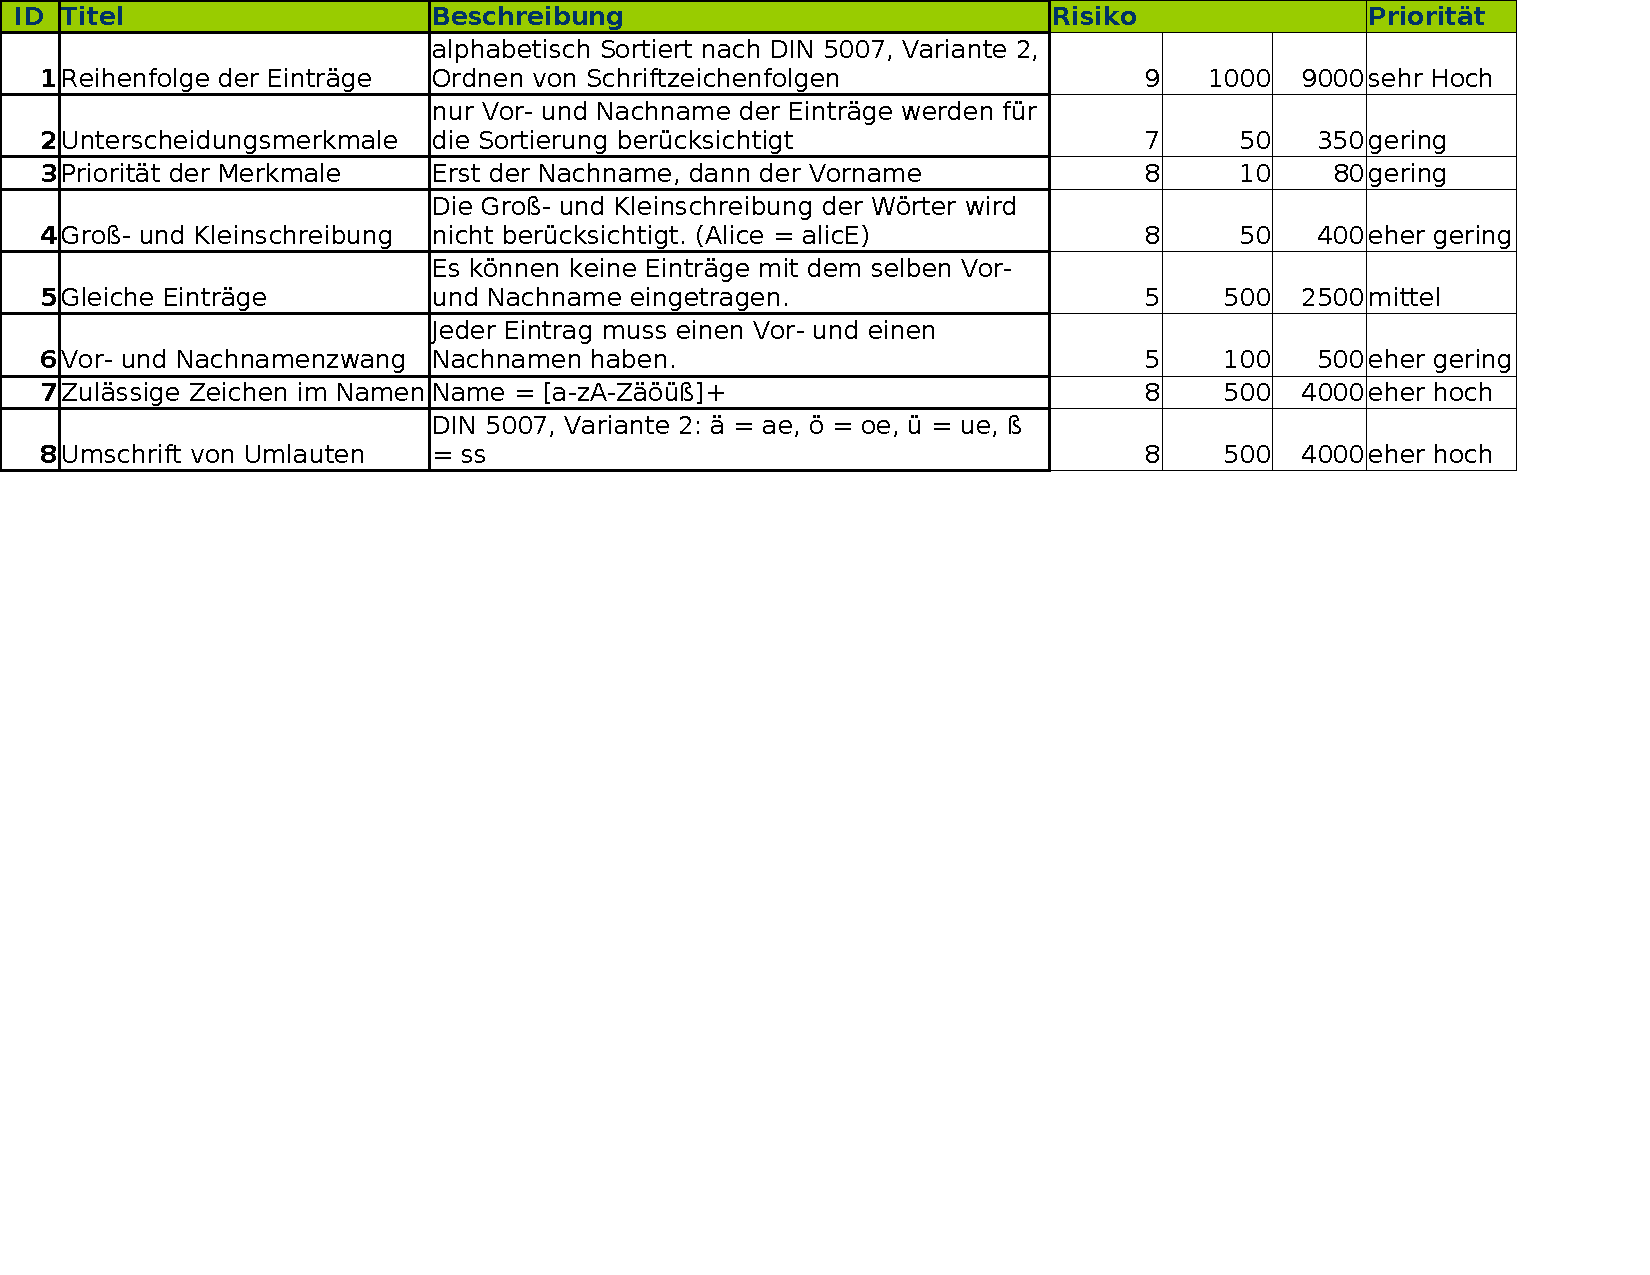
\includegraphics[width=1.4\linewidth]{Aufgabe2Tabelle}
%\begin{tabular}{rllll}
%ID & Titel & Beschreibung & Risiko & Priorität\\
%1 & Reihenfolge der Einträge & alphabetisch Sortiert nach DIN 5007, Variante 2, Ordnen von Schriftzeichenfolgen &  & \\
%2 & Unterscheidungsmerkmale & nur Vor- und Nachname der Einträge &  & \\
%3 & Priorität der Merkmale & Erst der Nachname, dann der Vornam &  & \\
%4 & Groß- und Kleinschreibung & Die Groß- und Kleinschreibung der Wörter wird nicht berücksichtigt. (Alice = alicE) &  & \\
%5 & Gleiche Einträge & Es können keine Einträge mit dem selben Vor- und Nachname eingetragen. &  & \\
%6 & Vor- und Nachnamenzwang & Jeder Eintrag muss einen Vor- und einen Nachnamen haben. &  & \\
%7 & Zulässige Zeichen im Namen & Name = [a-zA-Zäöüß]+ &  & \\
%8 & Umschrift von Umlauten & ä = ae, ö = oe, ü = ue, ß = ss &  & \\
%\end{tabular}
